% !TEX encoding = UTF-8 Unicode
\documentclass[a4paper]{article}

\usepackage{color}
\usepackage{url}
\usepackage[T2A]{fontenc} % enable Cyrillic fonts
\usepackage[utf8]{inputenc} % make weird characters work
\usepackage{graphicx}
\graphicspath{ {./images/} }
\usepackage{amsfonts}
\usepackage[english,serbian]{babel}
%\usepackage[english,serbianc]{babel} %ukljuciti babel sa ovim opcijama, umesto gornjim, ukoliko se koristi cirilica

\usepackage[unicode]{hyperref}
\hypersetup{colorlinks,citecolor=green,filecolor=green,linkcolor=blue,urlcolor=blue}

\usepackage{listings}
\usepackage{mathtools}
\usepackage{dirtytalk}
\usepackage{epigraph}


%\newtheorem{primer}{Пример}[section] %ćirilični primer
\newtheorem{primer}{Primer}[section]

\definecolor{mygreen}{rgb}{0,0.6,0}
\definecolor{mygray}{rgb}{0.5,0.5,0.5}
\definecolor{mymauve}{rgb}{0.58,0,0.82}

\lstset{ 
  backgroundcolor=\color{white},   % choose the background color; you must add \usepackage{color} or \usepackage{xcolor}; should come as last argument
  basicstyle=\scriptsize\ttfamily,        % the size of the fonts that are used for the code
  breakatwhitespace=false,         % sets if automatic breaks should only happen at whitespace
  breaklines=true,                 % sets automatic line breaking
  captionpos=b,                    % sets the caption-position to bottom
  commentstyle=\color{mygreen},    % comment style
  deletekeywords={...},            % if you want to delete keywords from the given language
  escapeinside={\%*}{*)},          % if you want to add LaTeX within your code
  extendedchars=true,              % lets you use non-ASCII characters; for 8-bits encodings only, does not work with UTF-8
  firstnumber=1000,                % start line enumeration with line 1000
  frame=single,	                   % adds a frame around the code
  keepspaces=true,                 % keeps spaces in text, useful for keeping indentation of code (possibly needs columns=flexible)
  keywordstyle=\color{blue},       % keyword style
  language=Python,                 % the language of the code
  morekeywords={*,...},            % if you want to add more keywords to the set
  numbers=left,                    % where to put the line-numbers; possible values are (none, left, right)
  numbersep=5pt,                   % how far the line-numbers are from the code
  numberstyle=\tiny\color{mygray}, % the style that is used for the line-numbers
  rulecolor=\color{black},         % if not set, the frame-color may be changed on line-breaks within not-black text (e.g. comments (green here))
  showspaces=false,                % show spaces everywhere adding particular underscores; it overrides 'showstringspaces'
  showstringspaces=false,          % underline spaces within strings only
  showtabs=false,                  % show tabs within strings adding particular underscores
  stepnumber=2,                    % the step between two line-numbers. If it's 1, each line will be numbered
  stringstyle=\color{mymauve},     % string literal style
  tabsize=2,	                   % sets default tabsize to 2 spaces
  title=\lstname                   % show the filename of files included with \lstinputlisting; also try caption instead of title
}

\begin{document}

\title{Optimizacija rojem čestica\\ \small{Seminarski rad u okviru kursa\\Metodologija stručnog i naučnog rada\\ Matematički fakultet}}

\author{Nevena Soldat, Milena Kurtić, Tijana Živković, Ana Miloradović\protect\\
\small{\texttt{nevenasoldat@gmail.com,}  \texttt{mimikurtic67@gmail.com,}} \\ \small{\texttt{tijanazivkovic6@gmail.com,} \texttt{ana.miloradovic7@gmail.com}}}

%\date{9.~april 2015.}

\maketitle

\abstract{ Kennedy i Eberhart (2001): \\
\say{... gledamo u paradigmu koja je u svom začeću, puna potencijala i novih ideja i novih perspektiva... Istraživači u mnogim zemljama eksperimentišu sa rojevima čestica... Mnoga pitanja koja su postavljena još uvek nisu dobila dobar odgovor.}

U ovom radu opisaćemo osnovni algoritam za optimizaciju rojem čestica, kao i neke od postojećih varijacija. Objasnićemo jednostavnije algoritme sa jedinstvenim rešenjem, ali i neke naprednije. Tema će biti i socijalne strukture na kojima se on zasniva, kao i koje su moguće primene. 
}

\tableofcontents

\newpage

\section{Uvod}
\label{sec:uvod}

Inteligencija rojeva predstavlja jednu od pet glavnih paradigmi Računarske Inteligencije (Computation Intelligence - CI). Jedinke u okviru grupe (roja) dele prikupljene informacije u zajedničkom cilju da reše neki problem, koje se propagiraju kroz celu grupu tako da se problem rešava mnogo efikasnije nego što bi to mogla pojedinačna jedinka.
Prvi i dosta značajan doprinos u polju inteligencije rojeva imao je južnoafrički pesnik Eugene N Marais koji je proučavao socijalno ponašanje kako majmuna, tako i mrava. Posle njega, ranih 1990-ih godina, Marco Dorigo modeluje ponašanje kolonija mrava. Zatim, 1995, Eberhart i Kennedy razvijaju algoritam optimizacije rojem čestica, na osnovu posmatranog jata ptica.
Optimizacija rojem čestica (eng. Particle Swarm Optimization - PSO) je stohastička optmizaciona tehnika zasnovana na veoma inteligentnom kolektivnom ponašanju nekih organizama kao što su insekti, ptice i ribe. Algoritam optimizacije rojem čestica otkriven je sasvim slučajno od strane Eberharta i Kenedija, pri pokušaju da se na računaru simulira kretanje jata ptica. Prvobitna namera bila je da se grafički prikaže nepredvidiva koreografija jata ptica, sa ciljem da se otkriju obrasci koji omogućavaju pticama da lete sinhronizovano, i da zadrže optimalnu formaciju pri naglim promenama pravaca. Sada je cilj kreiranje jednostavnog i efikasnog optimizacionog algoritma. Od kada je prvi put predstavljen 1995. doživeo je niz poboljšanja i nastale su brojne varijacije ovog algoritma. 


\section{Algoritam za optimizaciju rojem čestica}
Kako bismo lakše razumeli algoritam možemo zamisliti roj pčela koje lete preko polja sa cvećem. Roj ima urođenu želju da pronađe poziciju gde je cveće najgušće raspoređeno. Takođe, pčele nemaju nikakvo znanje o polju na kom se nalaze. Tako počinju svoju pretragu u različitim smerovima. Svaka pčela pamti mesta na kojima je bila i na kojim je bilo najviše cveća, i tu informaciju može preneti komunikacijom sa ostatkom roja. Kako vreme prolazi, pčele biraju da li će se vratiti na svoje prethodno pronađene najbolje lokacije ili će ići ka lokacijama koje su dobile od ostalih pčela. One koje oklevaju će ići u oba pravca i nalaziće se negde između ciljanih lokacija, u zavisnosti od toga da li će socijalan uticaj biti dominantan ili ne. Povremeno, pčela može da preleti preko dela polja u kom se nalazi više cveća od do sad otkrivenih lokacija. Tada će se čitav roj povlačiti ka novootkrivenoj lokaciji.
\begin{figure}[htp]
    \centering
    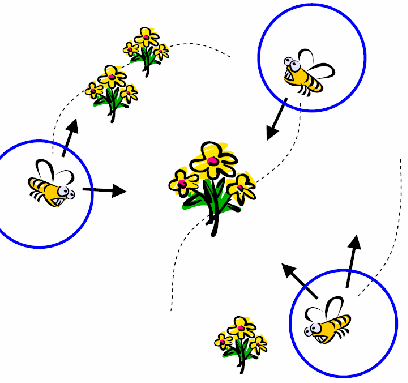
\includegraphics{bees.png}
    \caption{Prikaz PSO algoritma na kojem pčele traže cveće}
    \label{fig:bees}
\end{figure}
\\ \indent Na slici 1, isprekidane linije predstavljaju zamišljene putanje pčela, a strelice prikazuju dve komponente brzine (lokalno najbolju poziciju i globalno najbolju poziciju). Pčela u gornjem delu slike je pronašla globalno najbolju poziciju, dok je pčela sa leve strane pronašla lokalno najbolju poziciju. Pčela u donjem delu slike prikazuje da iako nije pronašla lokalno najbolju poziciju, ide ka globalno najboljoj poziciji. \\
\indent Na ovaj način pčele pretražuju polje tako što menjaju brzine i pravac kretanja u zavisnosti od toga da li je imala uspeha da pronađe cveće u odnosu na čitav roj. Takođe pčele znaju da izbegavaju mesta koja nisu imala puno cveća. Na kraju će pretražiti celo polje, i nalaziće se iznad mesta na kojem je najveća gustina cveća.

\subsection{Originalni PSO}
Algoritam za optimizaciju rojem čestica sadrži jedinke (čestice) koje se se kreću kroz višedimenzioni prostor pretrage, a pozicije jedinki se menjaju u skladu sa sopstvenim iskustvom, kao i sa iskustvom susednih jedinki. Svaka od tih čestica predstavlja jedno moguće rešenje.
Neka je $x_i(t)$ pozicija čestice \textit{i} u prostoru pretrage u trenutku \textit{t}. Pozicija čestice se menja dodavanjem brzine, $v_i(t)$ na trenutnu poziciju. \[x_i(t+1) = x_i(t) + v_i(t+1) \]
Njihovo kretanje se usmerava imajući u vidu njihovu trenutnu poziciju, njihovu do sada najbolju poziciju, kao i do sada najbolju poziciju čitavog roja. Kognitivna komponenta algoritma predstavlja tendenciju vraćanja u lično najbolje rešenje, dok socijalna komponenta predstavlja tendenciju ka globalno najboljem rešenju. Brzina se računa kao: \[ v_i(t+1) = v_i(t) + c_1r_1(p_i(t) - x_i(t)) + c_2r_2(p_g(t) - x_i(t))\]
gde $p_i(t)$ predstavlja najbolju do sada poziciju čestice \textit{i} u trenutku t, dok je $p_g(t)$ globalno najbolje rešenje (pozicija) do trenutka t. Parametri $r_1$ i $r_2$ su nasumične vrednosti izabrane iz uniformne raspodele na intervalu [0,1], dok su parametri $c_1$ i $c_2$ konstante koje predstavljaju pozitivna ubrzanja čija je uloga da skaliraju značaj kognitivne, odnosno socijalne komponente brzine. 

\subsection{Komponente brzine PSO algoritma}



\subsection{Globalno najbolji PSO}
\label{subsec:podnaslov1}

U slučaju globalno najboljeg PSO algoritma, susedi za svaku česticu su zapravo čitav roj. On implementira topologiju zvezde. U topologiji zvezde socijalna komponenta brzine čestice predstavlja informaciju dobijenu od svih čestica u roju. 
Brzina čestice i se računa kao:
\[v_{ij}(t + 1) = v_{ij}(t) + c_1r_{1j}(t)[y_{ij}(t) - x_{ij}(t)] + c_2r_{2j}(t)[\hat{y}_j(t) - x_{ij}(t)] \]

gde je $v_{ij}(t)$ brzina čestice \textit{i} u dimenziji \textit{j} = 1,...,$n_x$ u trenutku \textit{t}, $x_{ij}(t)$ je pozicija čestice \textit{i} u dimenziji \textit{j} u trenutku \textit{t}, $c_1$ i $c_2$ su konstante koje predstavljaju pozitivna ubrzanja čija je uloga da skaliraju značaj kognitivne, odnosno socijalne komponente brzine, i $r_{1j}(t)$, $r_{2j}(t)$ su nasumične vrednosti izabrane iz uniformne raspodele na intervalu [0,1].
Lokalno najbolje rešenje, $\textbf{y}_i$ je najbolja pozicija u kojoj je bila čestica \textit{i} od početnog trenutka \textit{t}. U trenutku \textit{t+1}, lokalno najbolje rešenje se računa na sledeći način:
\begin{equation}
    y_i(t+1) = \begin{cases}
                
            y_i(t)  & f(x_i(t+1)) \geq f(y_i(t)) \\
            x_i(t+1)  & f(x_i(t+1)) < f(y_i(t))
           
             \end{cases}
\end{equation}
gde je $f:\mathbb{R}^{n_x} \to \mathbb{R}$ fitnes funkcija. Fitnes funkcija računa koliko je dobijeno rešenje blisko optimalnom, odnosno meri kvalitet rešenja. Globalno najbolje rešenje, odnosno pozicija, u trenutku t, je definisano kao
\[\hat{y}(t) \in {y_0(t),...,y_{n_s}|f(\hat{y}(t)) = min{f(y_0(t)),...,f(y_{n_s}(t))}} \]
gde je $n_s$ ukupan broj čestica. Bitno je napomenutni da je $\hat{y}$ najbolje rešenje koje je pronađeno od strane bilo koje čestice do sada - obično se računa kao najbolje lokalno najbolje rešenje. Globalno najbolje rešenje se takođe može izabrati i od čestica posmatranog roja, u kom slučaju je \[\hat{y}(t) = min{f(x_0(t)),...,f(x_{n_s}(t))}\]
Globalno najbolji PSO je prikazan u narednom algoritmu \\ \\
\textbf{Algoritam} \textit{gbest} PSO: \\ 
Kreiraj i inicijalizuj $n_s$ - dimenzioni roj;\\
\textbf{ponavljaj} \\ 
\hspace*{5mm}\textbf{za} \textit{svaku česticu} $\textit{i} = 1,...,n_s$ \textbf{uradi} \\
\hspace*{5mm} // postavi lokalno najbolju poziciju \\
\hspace*{10mm} \textbf{ako} $f(x_i) < f(y_i)$ \textbf{onda} \\
\hspace*{15mm} $y_i = x_i;$ \\
\hspace*{10mm} \textbf{kraj} \\
\hspace*{5mm}//postavi globalno najbolju poziciju \\\
\hspace*{10mm}\textbf{ako} $f(y_i) < f(\hat{y})$ \textbf{onda} \\
\hspace*{15mm} $\hat{y} = y_i;$ \\
\hspace*{10mm} \textbf{kraj} \\
\hspace*{5mm} \textbf{kraj} \\
\hspace*{5mm} \textbf{za} \textit{svaku česticu} $i = 1,...,n_s$ \textbf{uradi}\\
\hspace*{10mm} ažuriraj brzinu; \\
\hspace*{10mm} ažiriraj poziciju; \\
\hspace*{5mm} \textbf{kraj} \\
\textbf{dok} nije ispunjen zahtev za zaustavljanje;



\subsection{Lokalno najbolji PSO}
\label{subsec:podnaslov2}

Lokalno najbolji PSO koristi topologiju prstena, gde svaka čestica i manji broj suseda. Socijalna komponenta predstavlja informaciju koju razmenjuju susedi čestice. Doprinos jedinke brzini je proporcionalna razdaljini između čestice i najbolje pozicije koju su pronašli susedi. Brzina se računa kao:
\[v_{ij}(t+1) = v_{ij}(t) + c_1r_{1j}(t)[y_{ij}(t) - x_{ij}(t)] + c_2r_{2j}(t)[\hat{y}_{ij}(t) - x_{ij}(t)] \]


\end{document}
